%%%%%%%%%%%%%%%%%%%%%%%%%%%%%%%%%%%%%%%%%%%%%%%%%%%%%%%%%%%%%%%%%%%%%%%%%%%%%%
%%%%%%%%%%%%%%%%%%%%%%%%%%%%%%%%%%%%%%%%%%%%%%%%%%%%%%%%%%%%%%%%%%%%%%%%%%%%%%
%%
%% Dokumentace k projektu pro předměty IFJ a IAL, 2012
%% Implementace interpretu imperativního jazyka IFJ12
%%
%%%%%%%%%%%%%%%%%%%%%%%%%%%%%%%%%%%%%%%%%%%%%%%%%%%%%%%%%%%%%%%%%%%%%%%%%%%%%%
%%%%%%%%%%%%%%%%%%%%%%%%%%%%%%%%%%%%%%%%%%%%%%%%%%%%%%%%%%%%%%%%%%%%%%%%%%%%%%
\documentclass[12pt,a4paper,titlepage,final]{article}

% matika
\usepackage[tbtags]{amsmath}
% cestina a fonty
\usepackage[czech]{babel}
\usepackage[utf8]{inputenc}
% balicky pro odkazy
\usepackage[bookmarksopen,colorlinks,plainpages=false,urlcolor=blue,unicode]{hyperref}
\usepackage{url}
% obrazky
\usepackage[dvipdf]{graphicx}
% velikost stranky
\usepackage[top=3.5cm, left=2.5cm, text={17cm, 24cm}, ignorefoot]{geometry}
\usepackage{lscape}

\begin{document}

%%%%%%%%%%%%%%%%%%%%%%%%%%%%%%%%%%%%%%%%%%%%%%%%%%%%%%%%%%%%%%%%%%%%%%%%%%%%%%
% titulní strana

\begin{titlepage}

% \vspace*{1cm}
\begin{figure}[!h]
  \centering
  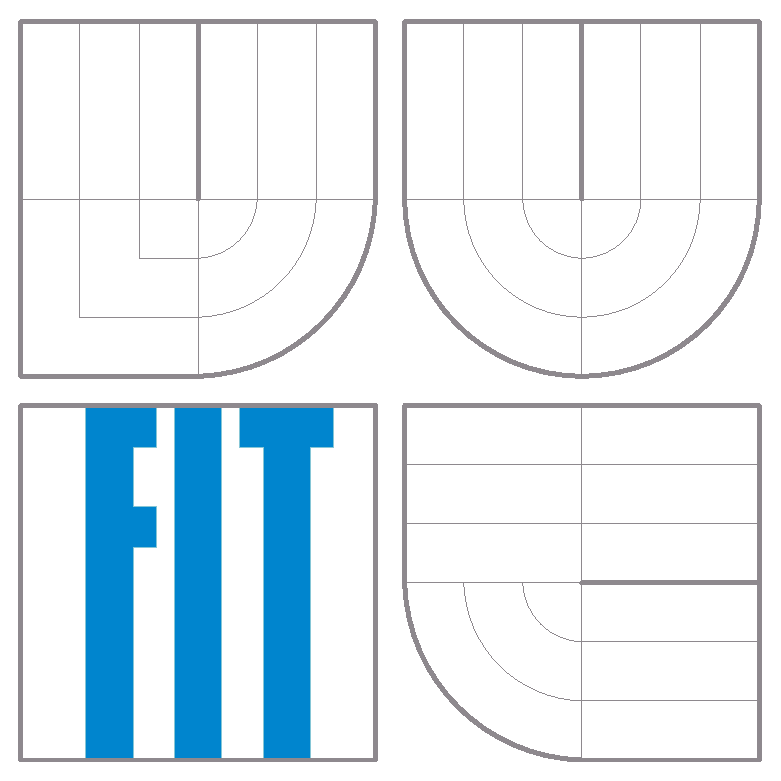
\includegraphics[height=5cm]{img/logo.eps} \\
  Fakulta Informačních Technologií \\
  Vysoké Učení Technické v~Brně
\end{figure}

\vfill

\begin{center}
\begin{Large}
Dokumentace k projektu pro předměty IFJ a IAL\\
\end{Large}
\bigskip
\begin{Huge}
Implementace interpretu imperativního jazyka IFJ12.\\
\end{Huge}
\end{center}

\vfill

\begin{center}
\begin{Large}
\today
\end{Large}
\end{center}

\vfill

\begin{flushleft}
\begin{large}
\begin{tabular}{l}
Tým 039, varianta a/4/I
\end{tabular}
\newline
\begin{tabular}{ll}
Rozšíření: & FUNEXP, LOGOP, MINUS
\end{tabular}
\newline
\newline
\begin{tabular}{llll}
% * @author Biberle Zdeněk <xbiber00@stud.fit.vutbr.cz>
% * @author Doležal Jan    <xdolez52@stud.fit.vutbr.cz>
% * @author Fryč Martin    <xfrycm01@stud.fit.vutbr.cz>
% * @author Kalina Jan     <xkalin03@stud.fit.vutbr.cz>
% * @author Tretter Zdeněk <xtrett00@stud.fit.vutbr.cz>
Autoři: & Zdeněk Biberle, & xbiber00 & 20\% \\
        & Jan Doležal,    & xdolez52 & 20\% \\
        & Martin Fryč,    & xfrycm01 & 20\% \\
        & Jan Kalina,     & xkalin03 & 20\% \\
        & Zdeněk Tretter, & xtrett00 & 20\% \\
\end{tabular}
\end{large}
\end{flushleft}
\end{titlepage}


%%%%%%%%%%%%%%%%%%%%%%%%%%%%%%%%%%%%%%%%%%%%%%%%%%%%%%%%%%%%%%%%%%%%%%%%%%%%%%
% obsah
\pagestyle{plain}
\pagenumbering{roman}
\setcounter{page}{1}
\tableofcontents

%%%%%%%%%%%%%%%%%%%%%%%%%%%%%%%%%%%%%%%%%%%%%%%%%%%%%%%%%%%%%%%%%%%%%%%%%%%%%%
% textova zprava
\newpage
\pagestyle{plain}
\pagenumbering{arabic}
\setcounter{page}{1}

%%%%%%%%%%%%%%%%%%%%%%%%%%%%%%%%%%%%%%%%%%%%%%%%%%%%%%%%%%%%%%%%%%%%%%%%%%%%%%
\section{Úvod} \label{uvod}
%%%%%%%%%%%%%%%%%%%%%%%%%%%%%%%%%%%%%%%%%%%%%%%%%%%%%%%%%%%%%%%%%%%%%%%%%%%%%%

Bla, bla, bla, bla, bla, bla, bla, bla, bla, bla, bla, bla, bla, bla, bla, bla,
bla, bla, bla, bla, bla, bla, bla, bla, bla, bla, bla, bla, bla, bla, bla, bla,
bla, bla, bla, bla, bla, bla, bla, bla, bla, bla, bla, bla, bla, bla, bla, bla...

%%%%%%%%%%%%%%%%%%%%%%%%%%%%%%%%%%%%%%%%%%%%%%%%%%%%%%%%%%%%%%%%%%%%%%%%%%%%%%
\section{Analýza problému a princip jeho řešení} \label{analyza}
%%%%%%%%%%%%%%%%%%%%%%%%%%%%%%%%%%%%%%%%%%%%%%%%%%%%%%%%%%%%%%%%%%%%%%%%%%%%%%

Bla, bla...

%=============================================================================
\subsection{Zadání problému}

Bla, bla...

%%%%%%%%%%%%%%%%%%%%%%%%%%%%%%%%%%%%%%%%%%%%%%%%%%%%%%%%%%%%%%%%%%%%%%%%%%%%%%
\section{Závěr} \label{zaver}
%%%%%%%%%%%%%%%%%%%%%%%%%%%%%%%%%%%%%%%%%%%%%%%%%%%%%%%%%%%%%%%%%%%%%%%%%%%%%%

Bla, bla...

%%%%%%%%%%%%%%%%%%%%%%%%%%%%%%%%%%%%%%%%%%%%%%%%%%%%%%%%%%%%%%%%%%%%%%%%%%%%%%
% seznam citované literatury: každá položka je definována příkazem
% \bibitem{xyz}, kde xyz je identifikátor citace (v textu použij: \cite{xyz})
\begin{thebibliography}{1}

% jedna citace:
\bibitem{kalendar}
BLACKBURN, B.~J.; HOLFORD-STREVENS, L.: \emph{The Oxford Companion to the
  Year}. Oxford: Oxford University Press, 1999, ISBN 0-19-214231-3.


\end{thebibliography}
%%%%%%%%%%%%%%%%%%%%%%%%%%%%%%%%%%%%%%%%%%%%%%%%%%%%%%%%%%%%%%%%%%%%%%%%%%%%%%
% přílohy
\appendix


\begin{landscape} % tabulku na sirku stranky
%%%%%%%%%%%%%%%%%%%%%%%%%%%%%%%%%%%%%%%%%%%%%%%%%%%%%%%%%%%%%%%%%%%%%%%%%%%%%%
\section{Příloha: Tabulka a pravidla precedenční syntaktické analýzy} \label{precedencnitabulka}
%%%%%%%%%%%%%%%%%%%%%%%%%%%%%%%%%%%%%%%%%%%%%%%%%%%%%%%%%%%%%%%%%%%%%%%%%%%%%%

\begin{minipage}{0.83\linewidth} % obal tabulky pro poznamky pod carou
\begin{large} % vetsi velikost pisma, aby tabulka vyplnila stranku
\begin{tabular}{|l|l|l|l|l|l|l|l|l|l|l|l|l|l|l|l|l|l|l|l|l|}
\hline
&+&-&*&/&**&(&)&\textless&\textgreater&\textless=&\textgreater=&!=& ==&in&notin&and&or&not&id&\$\\
\hline
+&\textgreater&\textgreater&\textless&\textless&\textless&\textless&\textgreater&\textgreater&\textgreater&\textgreater&\textgreater&\textgreater&\textgreater&\textgreater&\textgreater&\textgreater&\textgreater&\textgreater&\textless&\textgreater\\
\hline
-&\textgreater&\textgreater&\textless&\textless&\textless&\textless&\textgreater&\textgreater&\textgreater&\textgreater&\textgreater&\textgreater&\textgreater&\textgreater&\textgreater&\textgreater&\textgreater&\textgreater&\textless&\textgreater\\
\hline
*&\textgreater&\textgreater&\textgreater&\textgreater&\textless&\textless&\textgreater&\textgreater&\textgreater&\textgreater&\textgreater&\textgreater&\textgreater&\textgreater&\textgreater&\textgreater&\textgreater&\textgreater&\textless&\textgreater\\
\hline
/&\textgreater&\textgreater&\textgreater&\textgreater&\textless&\textless&\textgreater&\textgreater&\textgreater&\textgreater&\textgreater&\textgreater&\textgreater&\textgreater&\textgreater&\textgreater&\textgreater&\textgreater&\textless&\textgreater\\
\hline
**&\textgreater&\textgreater&\textgreater&\textgreater&\textgreater&\textless&\textgreater&\textgreater&\textgreater&\textgreater&\textgreater&\textgreater&\textgreater&\textgreater&\textgreater&\textgreater&\textgreater&\textgreater&\textless&\textgreater\\
\hline
(&\textless&\textless&\textless&\textless&\textless&\textless&=&\textless&\textless&\textless&\textless&\textless&\textless&\textless&\textless&\textless&\textless&\textless&\textless&\\
\hline
)&\textgreater&\textgreater&\textgreater&\textgreater&\textgreater&&\textgreater&\textgreater&\textgreater&\textgreater&\textgreater&\textgreater&\textgreater&\textgreater&\textgreater&\textgreater&\textgreater&\textgreater&&\textgreater\\
\hline
\textless&\textless&\textless&\textless&\textless&\textless&\textless&\textgreater&\textgreater&\textgreater&\textgreater&\textgreater&\textgreater&\textgreater&\textgreater&\textgreater&\textgreater&\textgreater&\textgreater&\textless&\textgreater\\
\hline
\textgreater&\textless&\textless&\textless&\textless&\textless&\textless&\textgreater&\textgreater&\textgreater&\textgreater&\textgreater&\textgreater&\textgreater&\textgreater&\textgreater&\textgreater&\textgreater&\textgreater&\textless&\textgreater\\
\hline
\textless=&\textless&\textless&\textless&\textless&\textless&\textless&\textgreater&\textgreater&\textgreater&\textgreater&\textgreater&\textgreater&\textgreater&\textgreater&\textgreater&\textgreater&\textgreater&\textgreater&\textless&\textgreater\\
\hline
\textgreater=&\textless&\textless&\textless&\textless&\textless&\textless&\textgreater&\textgreater&\textgreater&\textgreater&\textgreater&\textgreater&\textgreater&\textgreater&\textgreater&\textgreater&\textgreater&\textgreater&\textless&\textgreater\\
\hline
!=&\textless&\textless&\textless&\textless&\textless&\textless&\textgreater&\textgreater&\textgreater&\textgreater&\textgreater&\textgreater&\textgreater&\textgreater&\textgreater&\textgreater&\textgreater&\textgreater&\textless&\textgreater\\
\hline
 ==&\textless&\textless&\textless&\textless&\textless&\textless&\textgreater&\textgreater&\textgreater&\textgreater&\textgreater&\textgreater&\textgreater&\textgreater&\textgreater&\textgreater&\textgreater&\textgreater&\textless&\textgreater\\
\hline
in&\textless&\textless&\textless&\textless&\textless&\textless&\textgreater&\textgreater&\textgreater&\textgreater&\textgreater&\textgreater&\textgreater&\textgreater&\textgreater&\textgreater&\textgreater&\textgreater&\textless&\textgreater\\
\hline
notin&\textless&\textless&\textless&\textless&\textless&\textless&\textgreater&\textgreater&\textgreater&\textgreater&\textgreater&\textgreater&\textgreater&\textgreater&\textgreater&\textgreater&\textgreater&\textgreater&\textless&\textgreater\\
\hline
and&\textless&\textless&\textless&\textless&\textless&\textless&\textgreater&\textless&\textless&\textless&\textless&\textless&\textless&\textless&\textless&\textgreater&\textgreater&\textless&\textless&\textgreater\\
\hline
or&\textless&\textless&\textless&\textless&\textless&\textless&\textgreater&\textless&\textless&\textless&\textless&\textless&\textless&\textless&\textless&\textgreater&\textgreater&\textless&\textless&\textgreater\\
\hline
not&\textless&\textless&\textless&\textless&\textless&\textless&\textgreater&\textless&\textless&\textless&\textless&\textless&\textless&\textless&\textless&\textgreater&\textgreater&\textless&\textless&\textgreater\\
\hline
id&\textgreater&\textgreater&\textgreater&\textgreater&\textgreater&*&\textgreater&\textgreater&\textgreater&\textgreater&\textgreater&\textgreater&\textgreater&\textgreater&\textgreater&\textgreater&\textgreater&\textgreater&&\textgreater\\
\hline
-&\textgreater&\textgreater&\textgreater&\textgreater&\textgreater&\textless&\textgreater&\textgreater&\textgreater&\textgreater&\textgreater&\textgreater&\textgreater&\textgreater&\textgreater&\textgreater&\textgreater&\textgreater&\textless&\textgreater\\
\hline
\$&\textless&\textless&\textless&\textless&\textless&\textless&&\textless&\textless&\textless&\textless&\textless&\textless&\textless&\textless&\textless&\textless&\textless&\textless&\\
\hline
\end{tabular}

\end{large}
\end{minipage}
\qquad
\begin{minipage}{0.17\linewidth} % obal tabulky pro poznamky pod carou
\begin{math}
G = (N,T,P,E) \\
N = \{ E \} \\
T = \{ \\ +, -, *, /, **, (, ), <, >, <=, >=, \text{!=}, \text{==}, \text{in},
        \text{notin}, \text{and}, \text{or}, \text{not}, \text{i} \\ \} \\
P = \{ \\
1: E \rightarrow E + E \\
2: E \rightarrow E - E \\
3: E \rightarrow E * E \\
4: E \rightarrow E / E \\
5: E \rightarrow E ** E \\
6: E \rightarrow E < E \\
7: E \rightarrow E > E \\
8: E \rightarrow E <= E \\
9: E \rightarrow E >= E \\
10: E \rightarrow E \text{ != } E \\
11: E \rightarrow E \text{ == } E \\
12: E \rightarrow E \text{ in } E \\
13: E \rightarrow E \text{ notin } E \\
14: E \rightarrow E \text{ and } E \\
15: E \rightarrow E \text{ or } E \\
16: E \rightarrow \text{ not } E \\
17: E \rightarrow -E \\
18: E \rightarrow (E) \\
19: E \rightarrow \text{i} \\
\} \\ \\ \\
\end{math}
\end{minipage}
\end{landscape}

\begin{landscape} % tabulku na sirku stranky
%%%%%%%%%%%%%%%%%%%%%%%%%%%%%%%%%%%%%%%%%%%%%%%%%%%%%%%%%%%%%%%%%%%%%%%%%%%%%%
\section{Příloha: Rekurzivní sestup - LL(2) tabulka} \label{rekurzivnisestup}
%%%%%%%%%%%%%%%%%%%%%%%%%%%%%%%%%%%%%%%%%%%%%%%%%%%%%%%%%%%%%%%%%%%%%%%%%%%%%%

\begin{minipage}{\linewidth} % obal tabulky pro poznamky pod carou
\begin{large}

\begin{math}
G = (N,T,R,P) \\
N = \{ P, S, P', S', L, E', E \} \\
T = \{ =, [, ], \text{ i }, \text{ if }, \text{ else }, \text{ while }, \text{ end }, \text{ function }, (, ), \text{ , }, \text{ EOL } \} \\
\end{math}

\begin{minipage}{0.2\linewidth}
\begin{math}
1.  P  \rightarrow \varepsilon \\
2.  P  \rightarrow SP \\
3.  S  \rightarrow S' \\
4.  P' \rightarrow \varepsilon \\
5.  P' \rightarrow S'P' \\
6.  S' \rightarrow id = A \text{ EOL } \\
\end{math}
\end{minipage}
\begin{minipage}{0.42\linewidth}
\begin{math}
7.  A \rightarrow E \\
8.  A \rightarrow id[E':E'] \\
9.  S' \rightarrow \text{ if } E \text{ EOL } P' \text{ end } \text{ EOL } \\
10. S' \rightarrow \text{ while } E \text{ EOL } P' \text{ end } \text{ EOL } \\
11. S' \rightarrow \text{ return } E \text{ EOL } \\
12. S  \rightarrow \text{ function } id ( E' L ) \text{ EOL } P' \text{ end } \text{ EOL } \\
\end{math}
\end{minipage}
\begin{minipage}{0.4\linewidth}
\begin{math}
13. L  \rightarrow \varepsilon \\
14. L  \rightarrow E L \\
15. E' \rightarrow E \\
16. E' \rightarrow \varepsilon \\
\\ \\
\end{math}
\end{minipage}

\input{rectab.tex}
\end{large}
\end{minipage}
\end{landscape}

\end{document}
